\PassOptionsToPackage{unicode=true}{hyperref} % options for packages loaded elsewhere
\PassOptionsToPackage{hyphens}{url}
%
\documentclass[]{article}
\usepackage{lmodern}
\usepackage{amssymb,amsmath}
\usepackage{ifxetex,ifluatex}
\usepackage{fixltx2e} % provides \textsubscript
\ifnum 0\ifxetex 1\fi\ifluatex 1\fi=0 % if pdftex
  \usepackage[T1]{fontenc}
  \usepackage[utf8]{inputenc}
  \usepackage{textcomp} % provides euro and other symbols
\else % if luatex or xelatex
  \usepackage{unicode-math}
  \defaultfontfeatures{Ligatures=TeX,Scale=MatchLowercase}
\fi
% use upquote if available, for straight quotes in verbatim environments
\IfFileExists{upquote.sty}{\usepackage{upquote}}{}
% use microtype if available
\IfFileExists{microtype.sty}{%
\usepackage[]{microtype}
\UseMicrotypeSet[protrusion]{basicmath} % disable protrusion for tt fonts
}{}
\IfFileExists{parskip.sty}{%
\usepackage{parskip}
}{% else
\setlength{\parindent}{0pt}
\setlength{\parskip}{6pt plus 2pt minus 1pt}
}
\usepackage{hyperref}
\hypersetup{
            pdfborder={0 0 0},
            breaklinks=true}
\urlstyle{same}  % don't use monospace font for urls
\usepackage[margin=1in]{geometry}
\usepackage{graphicx,grffile}
\makeatletter
\def\maxwidth{\ifdim\Gin@nat@width>\linewidth\linewidth\else\Gin@nat@width\fi}
\def\maxheight{\ifdim\Gin@nat@height>\textheight\textheight\else\Gin@nat@height\fi}
\makeatother
% Scale images if necessary, so that they will not overflow the page
% margins by default, and it is still possible to overwrite the defaults
% using explicit options in \includegraphics[width, height, ...]{}
\setkeys{Gin}{width=\maxwidth,height=\maxheight,keepaspectratio}
\setlength{\emergencystretch}{3em}  % prevent overfull lines
\providecommand{\tightlist}{%
  \setlength{\itemsep}{0pt}\setlength{\parskip}{0pt}}
\setcounter{secnumdepth}{0}
% Redefines (sub)paragraphs to behave more like sections
\ifx\paragraph\undefined\else
\let\oldparagraph\paragraph
\renewcommand{\paragraph}[1]{\oldparagraph{#1}\mbox{}}
\fi
\ifx\subparagraph\undefined\else
\let\oldsubparagraph\subparagraph
\renewcommand{\subparagraph}[1]{\oldsubparagraph{#1}\mbox{}}
\fi

% set default figure placement to htbp
\makeatletter
\def\fps@figure{htbp}
\makeatother

%latex header to wrap code lines in .pdf

\usepackage{fvextra}
\DefineVerbatimEnvironment{Highlighting}{Verbatim}{breaklines,commandchars=\\\{\}}

% To keep the figure from floating around
% All figures should be forced in-place via the [H]ERE float specification.
\usepackage{float}
\floatplacement{figure}{H}
%\floatplacement{figure}{!htbp}

\date{}

\begin{document}

\hypertarget{report-of-the-fit}{%
\section{Report of the fit}\label{report-of-the-fit}}

\hypertarget{fit-summary}{%
\subsection{Fit summary}\label{fit-summary}}

Description: MAP21 pion TMDs3\\
Minimiser: minuit\\
Random seed: 5814\\
Maximum values allowed for \(q_T / Q\): 0.3 \(+\) 0.6\(/ Q\) {]}\\
Percentile cut: 8\\
Parameterisation: MAPTMDPion3\\
Initial parameters fluctuations: True\\
Explicit formula:

\[f_{\rm NP}(x,\zeta, b_T)= \exp \left( g_{1\pi}(x) b_T^2 / 4 \right) \exp\left[- g^2_2 \log\left(\frac{\zeta}{Q_0^2}\right) b_T^2/4 \right]\]\[g_{1\pi}(x) = N_{1\pi} \frac{x^{\sigma_{\pi}}(1-x)^{\alpha^2_{\pi}}}{\hat{x}^{\sigma_{\pi}}(1-\hat{x})^{\alpha^2_{\pi}}}\]\[Q_0^2 = 1\;{\rm GeV}^2\]\[\hat{x} = 0.1\]
\(t_0\) prescription: False\\
\#\# Theory summary

Collinear PDF set: MMHT2014nnlo68cl member 0\\
Collinear pion PDF set: xFitterPI\_NLO\_EIG member 0\\
\(b^*\) prescription: bstarmin\\
Perturbative order: N3LL\\
Reference value of the fine-structure constant:
\(\alpha(Q = 91.1876\;{\rm GeV}) = 0.00776578395589\) (running True)

\hypertarget{global-statistical-estimators}{%
\subsection{Global statistical
estimators}\label{global-statistical-estimators}}

\(N_{rep}\) = 201\\
\(\chi_{0}^2\) = 1.5455\\
\(\chi_{mean}^2\) = 1.5509\\
\(\langle\chi^2\rangle \pm \sigma_{\chi^2}\) = 1.5746 \(\pm\) 0.0349\\
\(\langle E \rangle \pm \sigma_{E}\) = 2.5298 \(\pm\) 0.2367

\hypertarget{parameters}{%
\subsection{Parameters}\label{parameters}}

\begin{table}[h]

\centering

\begin{tabular}{|c|c|c|c|} \hline

\textbf{Parameter} & \textbf{Central replica} & \textbf{Average over
replicas} & \textbf{Fixed} \\ \hline

\(N_{1\pi}\) & 0.46913915 & 0.46515638 \(\pm\)
0.11839214 & False \\ \hline
\(\sigma_\pi\) & 4.0378396 & 4.49853325 \(\pm\)
2.24574404 & False \\ \hline
\(\alpha_\pi\) & 4.3688834 & 4.39661602 \(\pm\)
1.33581571 & False \\ \hline

\end{tabular}

\caption{}

\end{table}

\begin{figure}
\centering
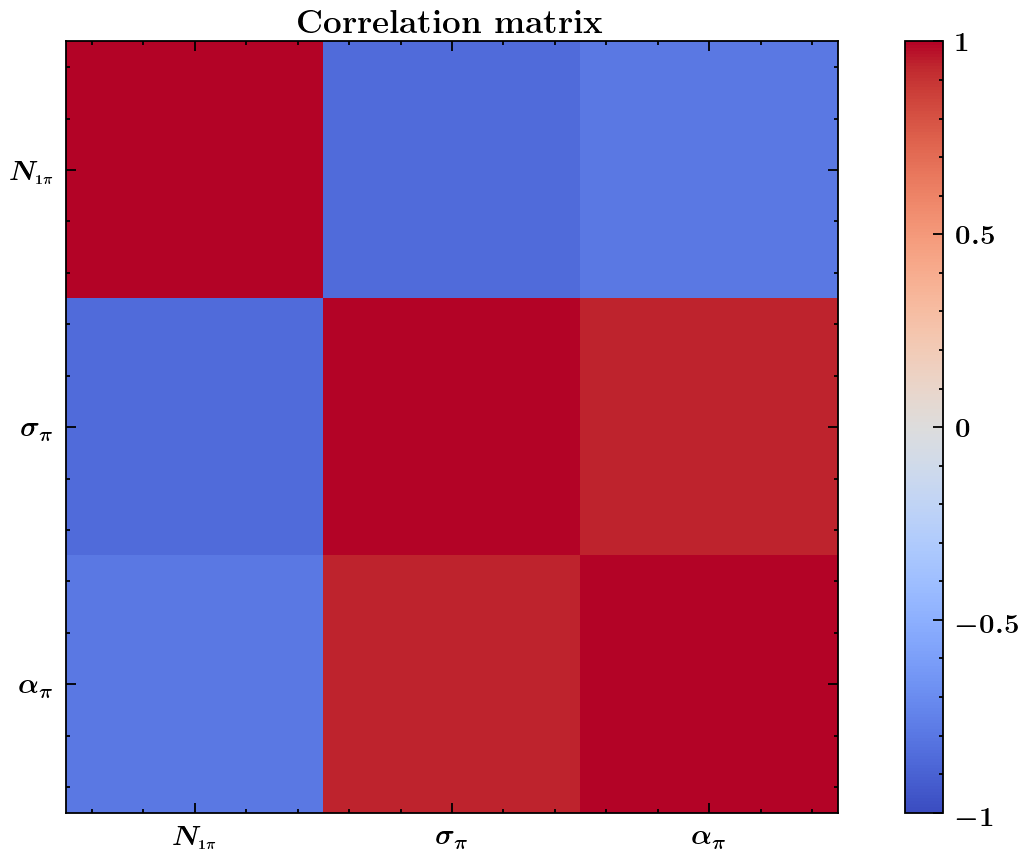
\includegraphics{pngplots/CorrelationMatrix.png}
\caption{Fitted parameter correlation matrix}
\end{figure}

\hypertarget{fit-properties}{%
\subsection{Fit properties}\label{fit-properties}}

\begin{figure}
\centering
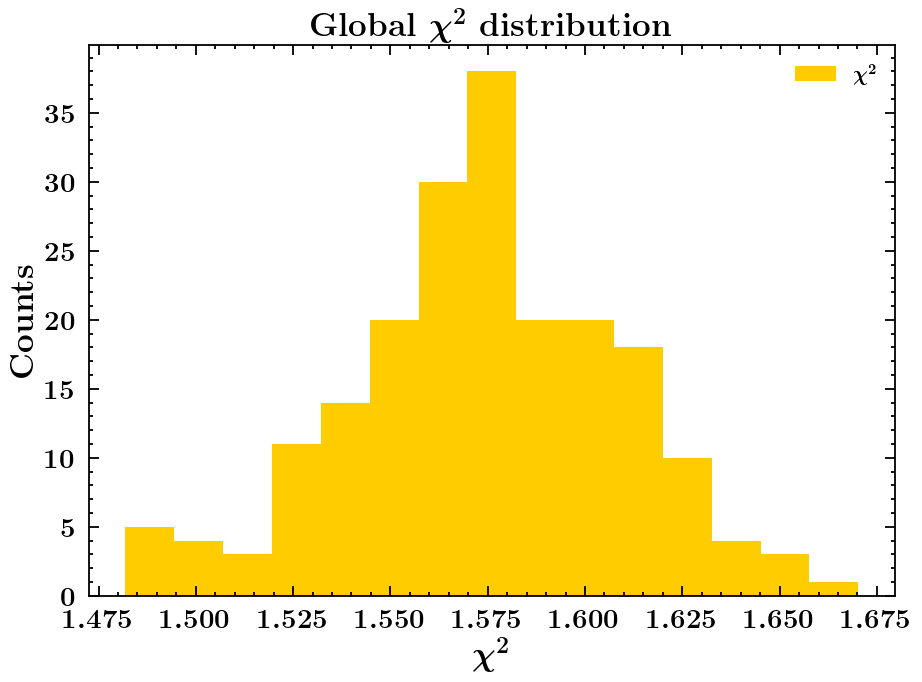
\includegraphics{pngplots/Globalchi2.png}
\caption{Global \(\chi^2\) distribution}
\end{figure}

\begin{figure}
\centering
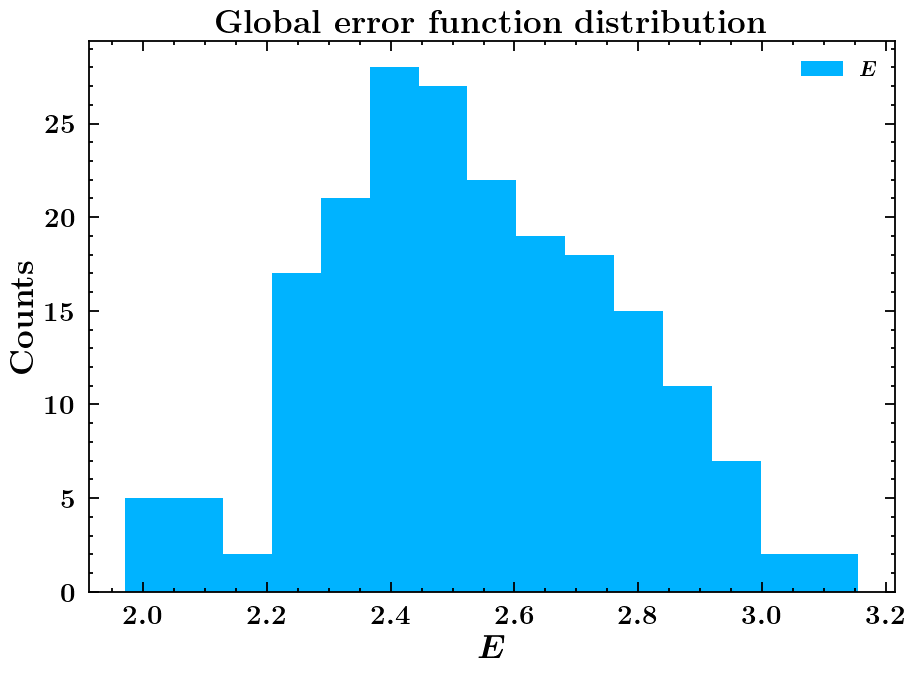
\includegraphics{pngplots/GlobalErrorFunction.png}
\caption{Global error function distribution}
\end{figure}

\begin{figure}
\centering
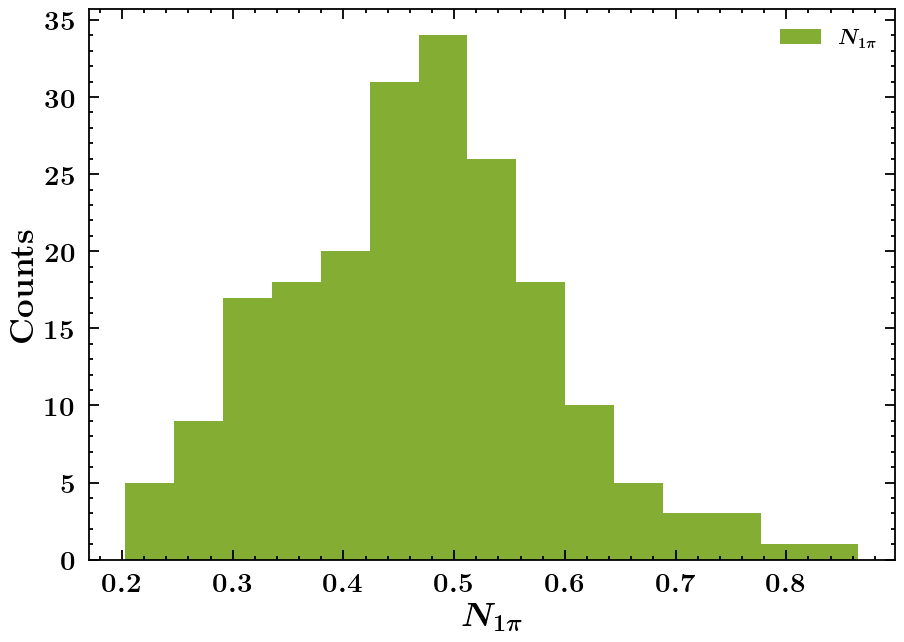
\includegraphics{pngplots/param0.png}
\caption{\(N_{1\pi}\) distribution}
\end{figure}

\begin{figure}
\centering
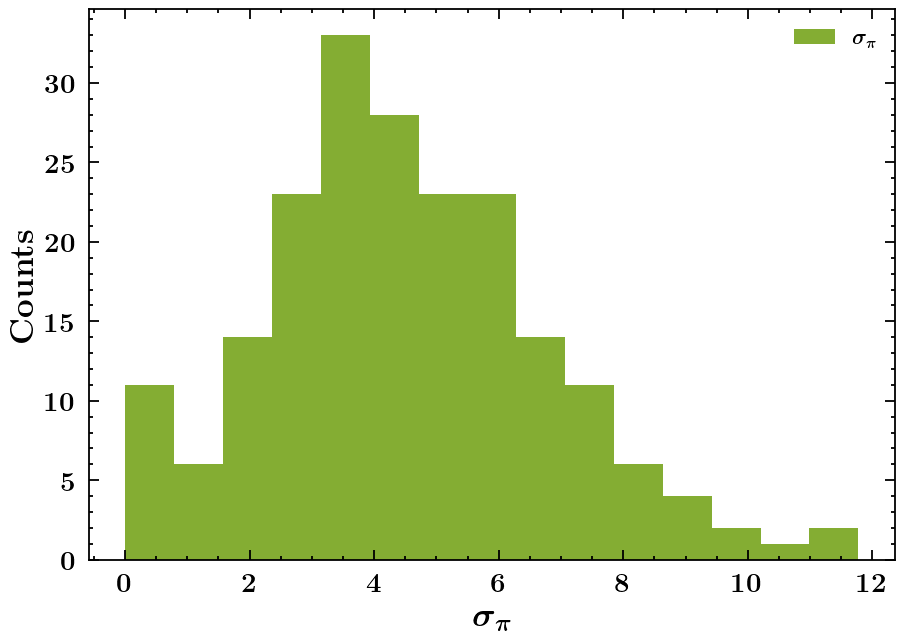
\includegraphics{pngplots/param1.png}
\caption{\(\sigma_\pi\) distribution}
\end{figure}

\begin{figure}
\centering
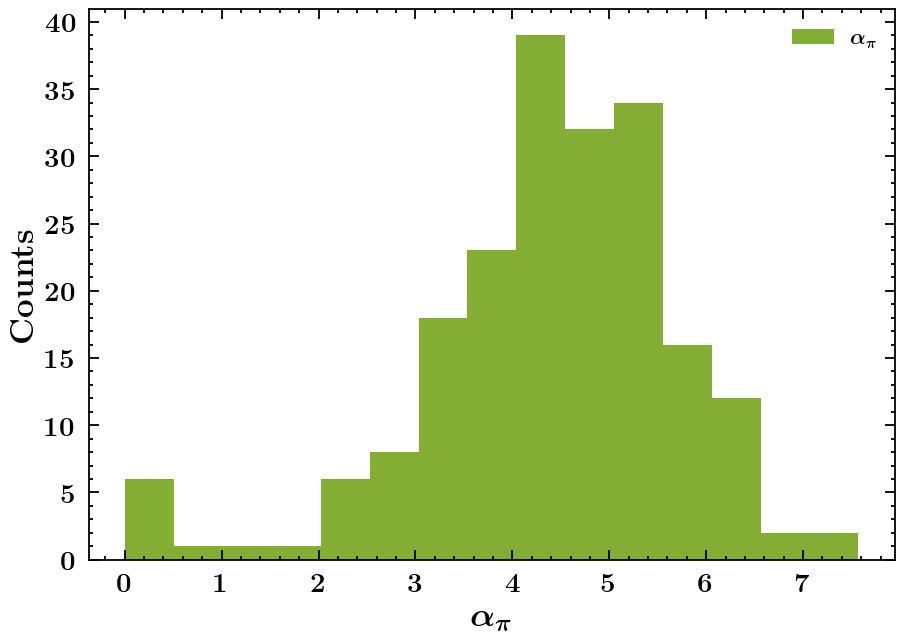
\includegraphics{pngplots/param2.png}
\caption{\(\alpha_\pi\) distribution}
\end{figure}

\hypertarget{table-of-chi2s}{%
\subsection{\texorpdfstring{Table of
\(\chi^2\)'s}{Table of \textbackslash{}chi\^{}2's}}\label{table-of-chi2s}}

\begin{table}[h]

\centering

\begin{tabular}{|c|c|c|c|c|} \hline

\textbf{Experiment} & \textbf{Number of
points} & \textbf{\(\chi_{D}^2\)} & \textbf{\(\chi_{\lambda}^2\)} & \textbf{\(\chi^2\)} \\ \hline

E537\_Q\_4.0\_4.5 & 6 & 0.604 & 0.773 & 1.377 \\ \hline
E537\_Q\_4.5\_5.0 & 7 & 1.147 & 1.549 & 2.696 \\ \hline
E537\_Q\_5.0\_5.5 & 8 & 1.223 & 1.01 & 2.233 \\ \hline
E537\_Q\_5.5\_6.0 & 7 & 1.733 & 0.699 & 2.432 \\ \hline
E537\_Q\_6.0\_6.5 & 9 & 1.038 & 0.377 & 1.415 \\ \hline
E537\_Q\_6.5\_7.0 & 9 & 0.926 & 0.179 & 1.105 \\ \hline
E537\_Q\_7.0\_7.5 & 7 & 0.82 & 0.156 & 0.976 \\ \hline
E537\_Q\_7.5\_8.0 & 6 & 0.751 & 0.16 & 0.911 \\ \hline
E537\_Q\_8.0\_8.5 & 2 & 0.687 & 0.04 & 0.727 \\ \hline
E537\_Q\_8.5\_9.0 & 3 & 0.412 & 0.04 & 0.452 \\ \hline
E615\_Q\_4.05\_4.50 & 7 & 0.706 & 1.453 & 2.158 \\ \hline
E615\_Q\_4.50\_4.95 & 8 & 0.57 & 1.175 & 1.745 \\ \hline
E615\_Q\_4.95\_5.40 & 8 & 0.128 & 1.321 & 1.45 \\ \hline
E615\_Q\_5.40\_5.85 & 9 & 0.135 & 1.271 & 1.406 \\ \hline
E615\_Q\_5.85\_6.75 & 9 & 0.187 & 1.442 & 1.629 \\ \hline
E615\_Q\_6.75\_7.65 & 10 & 0.157 & 1.45 & 1.607 \\ \hline
E615\_Q\_7.65\_9.00 & 12 & 0.357 & 1.436 & 1.793 \\ \hline
E615\_Q\_11.70\_13.05 & 11 & 0.364 & 0.355 & 0.719 \\ \hline
Total & 138 & 0.633 & 0.912 & 1.545 \\ \hline

\end{tabular}

\caption{Central-replica \(\chi^2\)'s:}

\end{table}

\begin{table}[h]

\centering

\begin{tabular}{|c|c|c|c|c|} \hline

\textbf{Experiment} & \textbf{Number of
points} & \textbf{\(\chi_{D}^2\)} & \textbf{\(\chi_{\lambda}^2\)} & \textbf{\(\chi^2\)} \\ \hline

E537\_Q\_4.0\_4.5 & 6 & 0.593 & 0.727 & 1.32 \\ \hline
E537\_Q\_4.5\_5.0 & 7 & 1.149 & 1.523 & 2.672 \\ \hline
E537\_Q\_5.0\_5.5 & 8 & 1.23 & 0.999 & 2.229 \\ \hline
E537\_Q\_5.5\_6.0 & 7 & 1.693 & 0.701 & 2.395 \\ \hline
E537\_Q\_6.0\_6.5 & 9 & 1.036 & 0.381 & 1.417 \\ \hline
E537\_Q\_6.5\_7.0 & 9 & 0.932 & 0.183 & 1.115 \\ \hline
E537\_Q\_7.0\_7.5 & 7 & 0.827 & 0.158 & 0.985 \\ \hline
E537\_Q\_7.5\_8.0 & 6 & 0.766 & 0.161 & 0.926 \\ \hline
E537\_Q\_8.0\_8.5 & 2 & 0.712 & 0.042 & 0.754 \\ \hline
E537\_Q\_8.5\_9.0 & 3 & 0.416 & 0.04 & 0.456 \\ \hline
E615\_Q\_4.05\_4.50 & 7 & 0.813 & 1.508 & 2.321 \\ \hline
E615\_Q\_4.50\_4.95 & 8 & 0.599 & 1.131 & 1.73 \\ \hline
E615\_Q\_4.95\_5.40 & 8 & 0.248 & 1.278 & 1.526 \\ \hline
E615\_Q\_5.40\_5.85 & 9 & 0.167 & 1.24 & 1.407 \\ \hline
E615\_Q\_5.85\_6.75 & 9 & 0.198 & 1.422 & 1.62 \\ \hline
E615\_Q\_6.75\_7.65 & 10 & 0.151 & 1.453 & 1.603 \\ \hline
E615\_Q\_7.65\_9.00 & 12 & 0.31 & 1.454 & 1.764 \\ \hline
E615\_Q\_11.70\_13.05 & 11 & 0.367 & 0.356 & 0.723 \\ \hline
Total & 138 & 0.645 & 0.905 & 1.551 \\ \hline

\end{tabular}

\caption{Mean-replica \(\chi^2\)'s:}

\end{table}

\begin{table}[h]

\centering

\begin{tabular}{|c|c|c|} \hline

\textbf{Experiment} & \textbf{Number of
points} & \textbf{\(\chi^2\)} \\ \hline

E537\_Q\_4.0\_4.5 & 6 & 1.445 \(\pm\) 0.154 \\ \hline
E537\_Q\_4.5\_5.0 & 7 & 2.736 \(\pm\) 0.147 \\ \hline
E537\_Q\_5.0\_5.5 & 8 & 2.267 \(\pm\) 0.086 \\ \hline
E537\_Q\_5.5\_6.0 & 7 & 2.469 \(\pm\) 0.099 \\ \hline
E537\_Q\_6.0\_6.5 & 9 & 1.448 \(\pm\) 0.049 \\ \hline
E537\_Q\_6.5\_7.0 & 9 & 1.132 \(\pm\) 0.035 \\ \hline
E537\_Q\_7.0\_7.5 & 7 & 0.999 \(\pm\) 0.032 \\ \hline
E537\_Q\_7.5\_8.0 & 6 & 0.928 \(\pm\) 0.022 \\ \hline
E537\_Q\_8.0\_8.5 & 2 & 0.742 \(\pm\) 0.036 \\ \hline
E537\_Q\_8.5\_9.0 & 3 & 0.457 \(\pm\) 0.006 \\ \hline
E615\_Q\_4.05\_4.50 & 7 & 2.193 \(\pm\) 0.157 \\ \hline
E615\_Q\_4.50\_4.95 & 8 & 1.754 \(\pm\) 0.111 \\ \hline
E615\_Q\_4.95\_5.40 & 8 & 1.478 \(\pm\) 0.091 \\ \hline
E615\_Q\_5.40\_5.85 & 9 & 1.444 \(\pm\) 0.053 \\ \hline
E615\_Q\_5.85\_6.75 & 9 & 1.67 \(\pm\) 0.05 \\ \hline
E615\_Q\_6.75\_7.65 & 10 & 1.637 \(\pm\) 0.041 \\ \hline
E615\_Q\_7.65\_9.00 & 12 & 1.823 \(\pm\) 0.078 \\ \hline
E615\_Q\_11.70\_13.05 & 11 & 0.722 \(\pm\) 0.006 \\ \hline
Total & 138 & 1.575 \(\pm\) 0.035 \\ \hline

\end{tabular}

\caption{Average-over-replicas \(\chi^2\)'s:}

\end{table}

\hypertarget{tmds-in-k_t-space}{%
\subsection{\texorpdfstring{TMDs in \(k_T\)
space}{TMDs in k\_T space}}\label{tmds-in-k_t-space}}

\begin{figure}
\centering
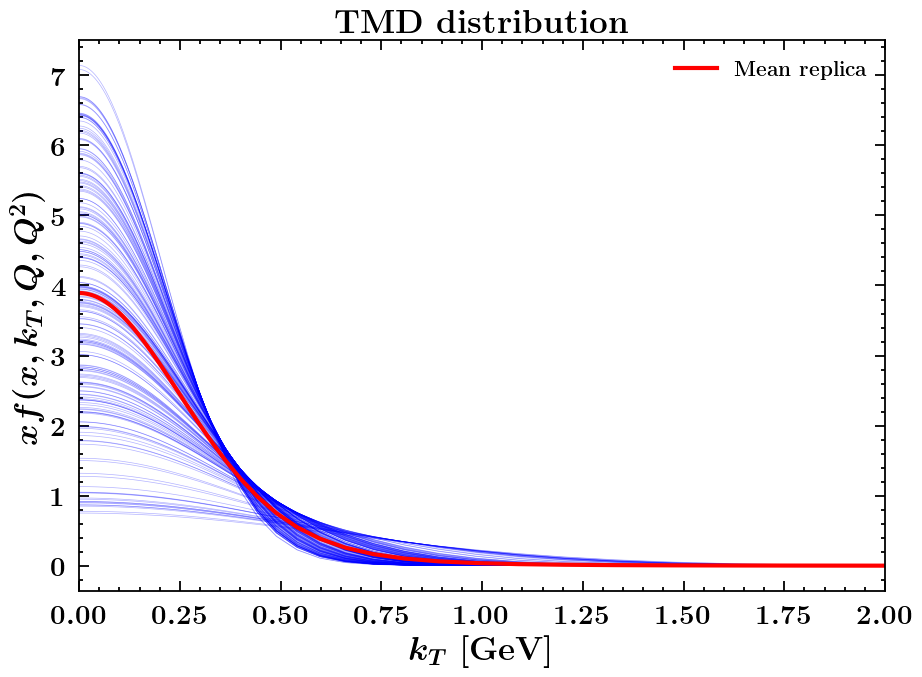
\includegraphics{pngplots/tmd_1_2_0.05.png}
\caption{TMD PDFBEAM of the \(d\) at \(Q = 2\) GeV and \(x = 0.05\)}
\end{figure}

\begin{figure}
\centering
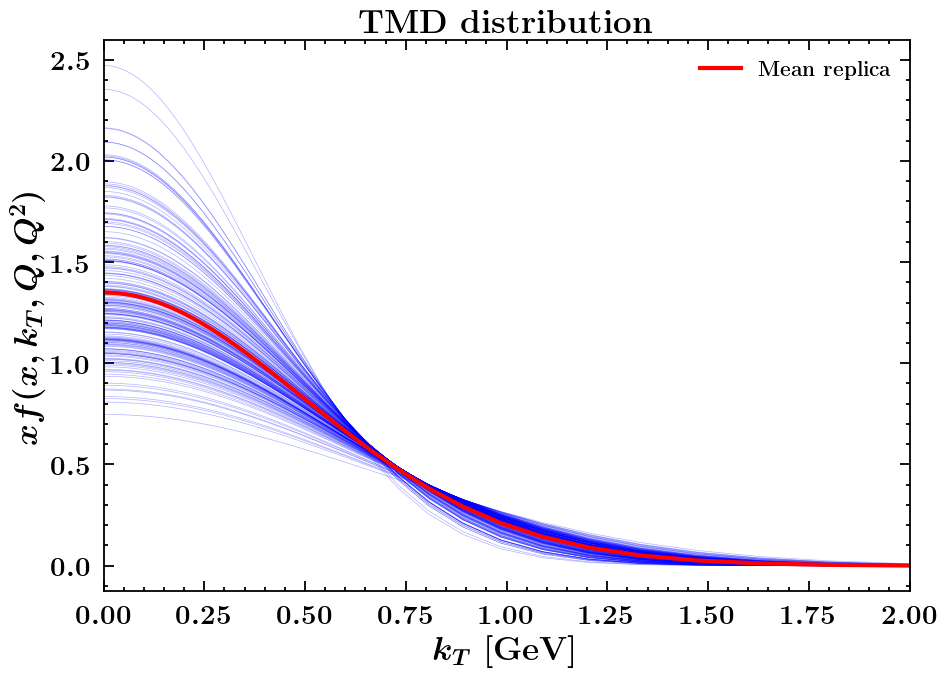
\includegraphics{pngplots/tmd_1_2_0.1.png}
\caption{TMD PDFBEAM of the \(d\) at \(Q = 2\) GeV and \(x = 0.1\)}
\end{figure}

\begin{figure}
\centering
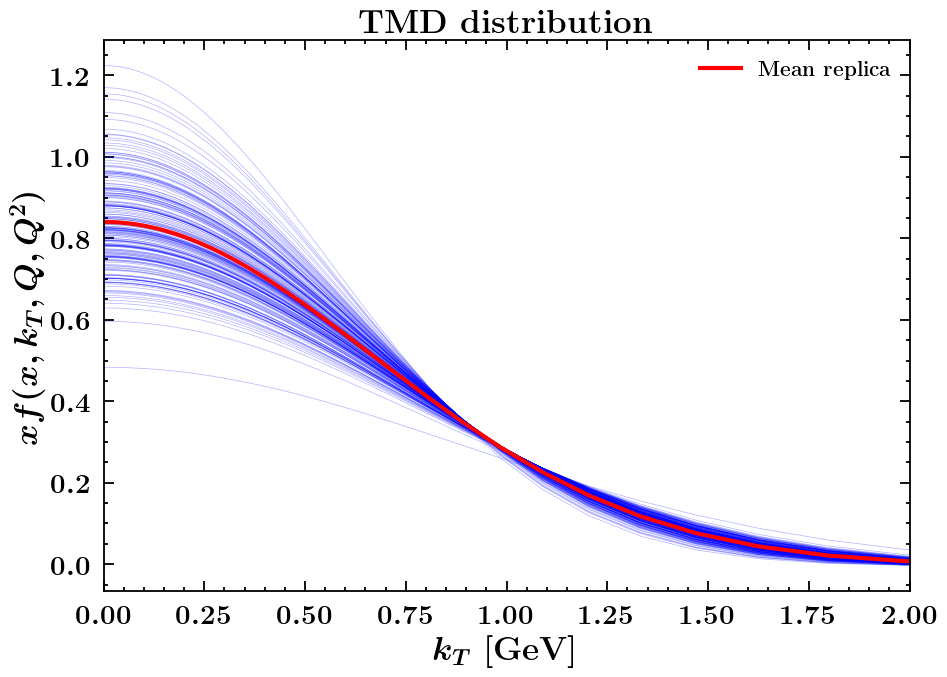
\includegraphics{pngplots/tmd_1_2_0.2.png}
\caption{TMD PDFBEAM of the \(d\) at \(Q = 2\) GeV and \(x = 0.2\)}
\end{figure}

\begin{figure}
\centering
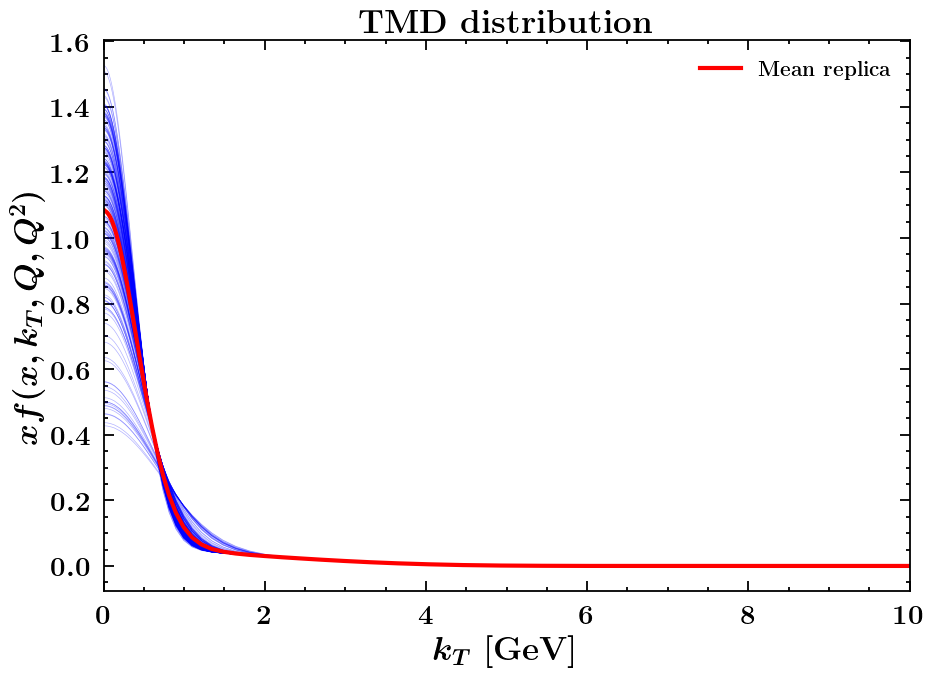
\includegraphics{pngplots/tmd_1_10_0.05.png}
\caption{TMD PDFBEAM of the \(d\) at \(Q = 10\) GeV and \(x = 0.05\)}
\end{figure}

\begin{figure}
\centering
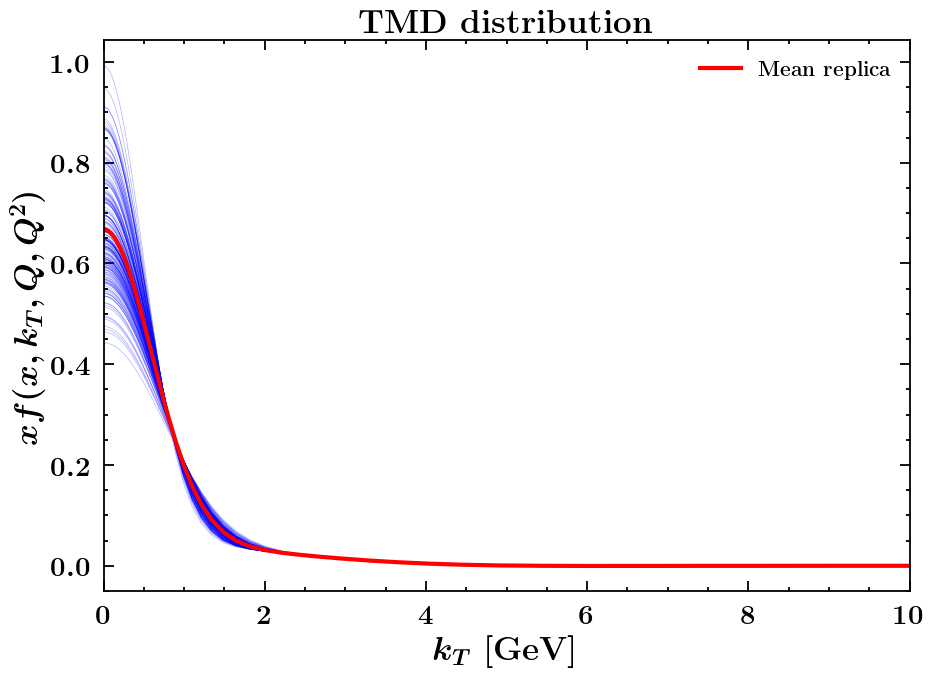
\includegraphics{pngplots/tmd_1_10_0.1.png}
\caption{TMD PDFBEAM of the \(d\) at \(Q = 10\) GeV and \(x = 0.1\)}
\end{figure}

\begin{figure}
\centering
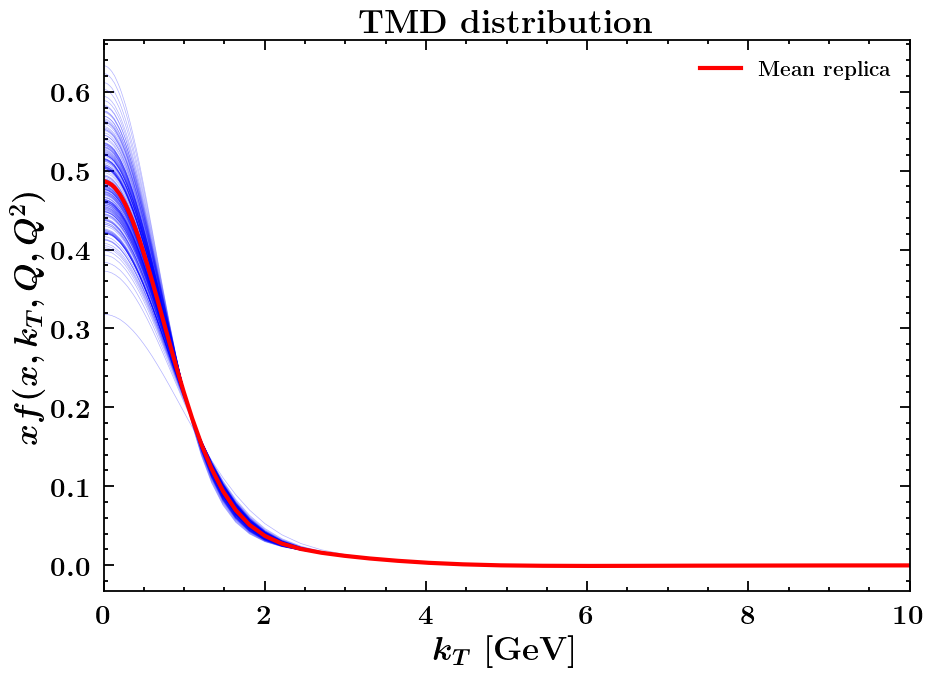
\includegraphics{pngplots/tmd_1_10_0.2.png}
\caption{TMD PDFBEAM of the \(d\) at \(Q = 10\) GeV and \(x = 0.2\)}
\end{figure}

\hypertarget{data-theory-comparison}{%
\subsection{Data-theory comparison}\label{data-theory-comparison}}

\begin{figure}
\centering
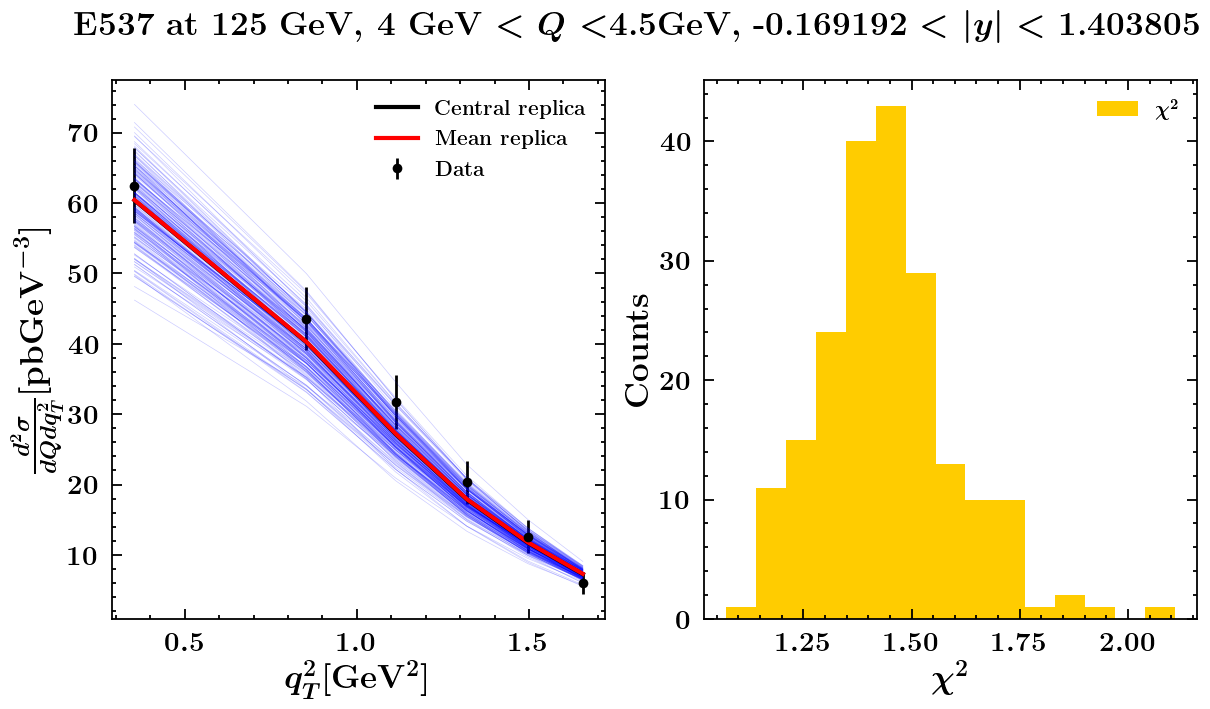
\includegraphics{pngplots/E537_Q_4.0_4.5.png}
\caption{E537\_Q\_4.0\_4.5 data-theory comparison}
\end{figure}

\begin{figure}
\centering
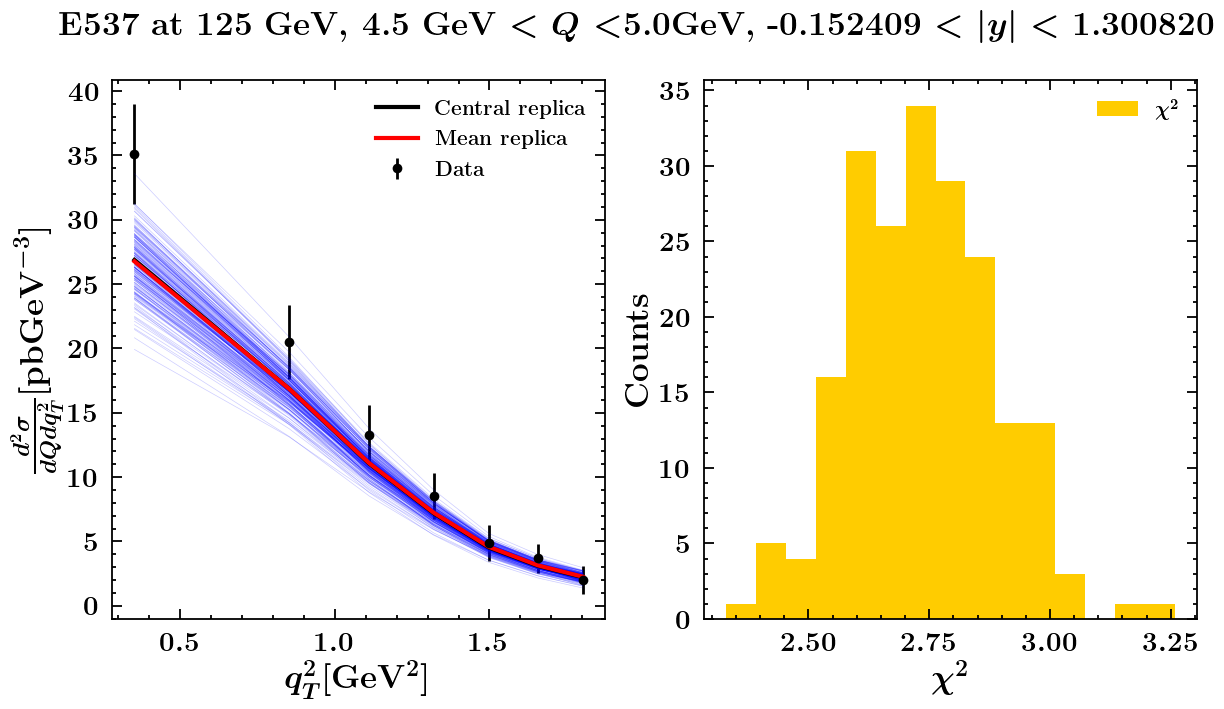
\includegraphics{pngplots/E537_Q_4.5_5.0.png}
\caption{E537\_Q\_4.5\_5.0 data-theory comparison}
\end{figure}

\begin{figure}
\centering
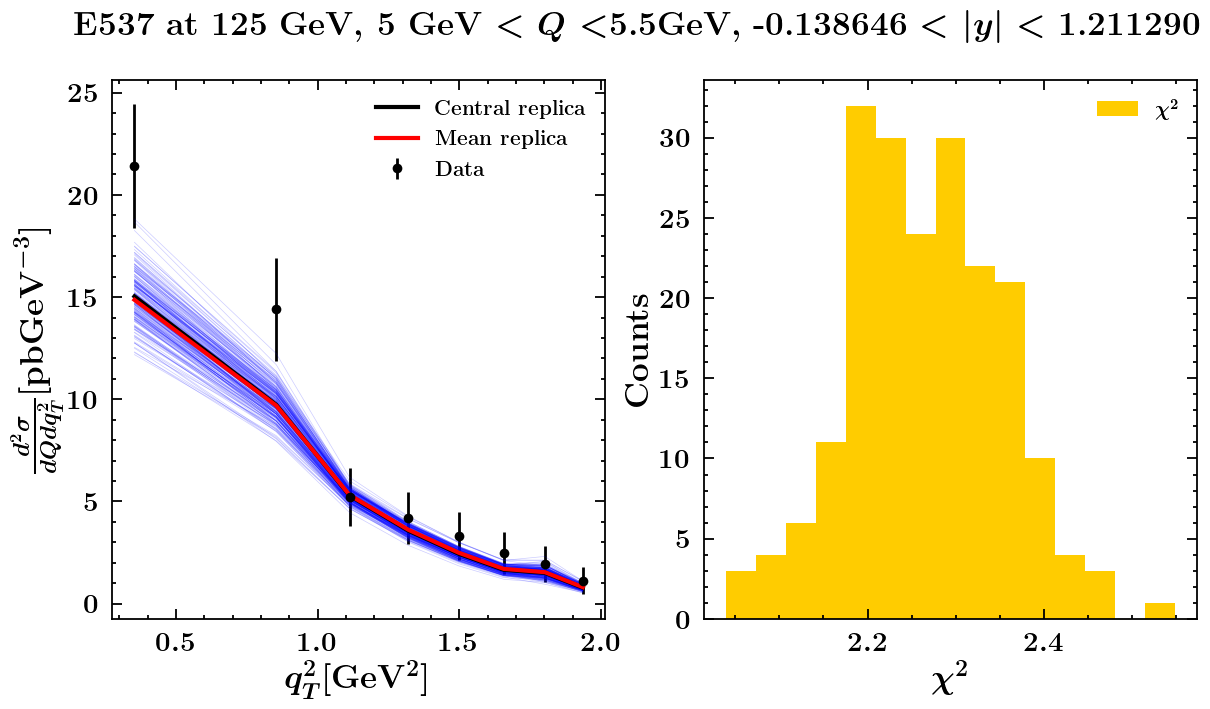
\includegraphics{pngplots/E537_Q_5.0_5.5.png}
\caption{E537\_Q\_5.0\_5.5 data-theory comparison}
\end{figure}

\begin{figure}
\centering
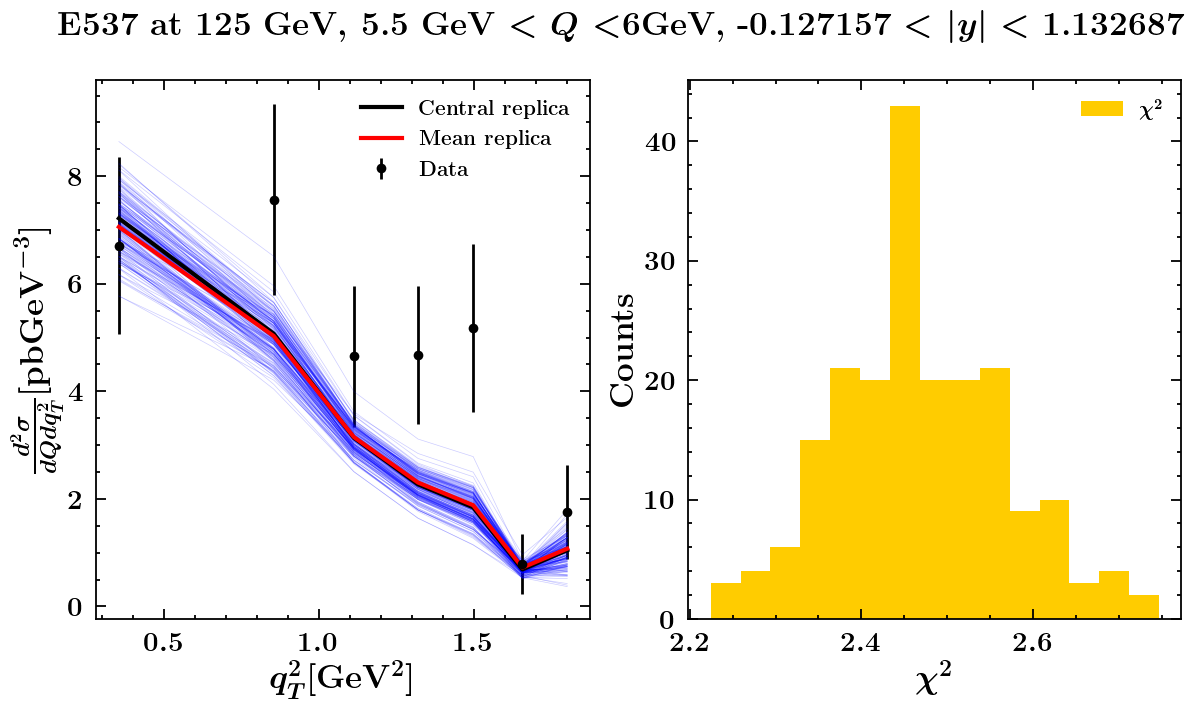
\includegraphics{pngplots/E537_Q_5.5_6.0.png}
\caption{E537\_Q\_5.5\_6.0 data-theory comparison}
\end{figure}

\begin{figure}
\centering
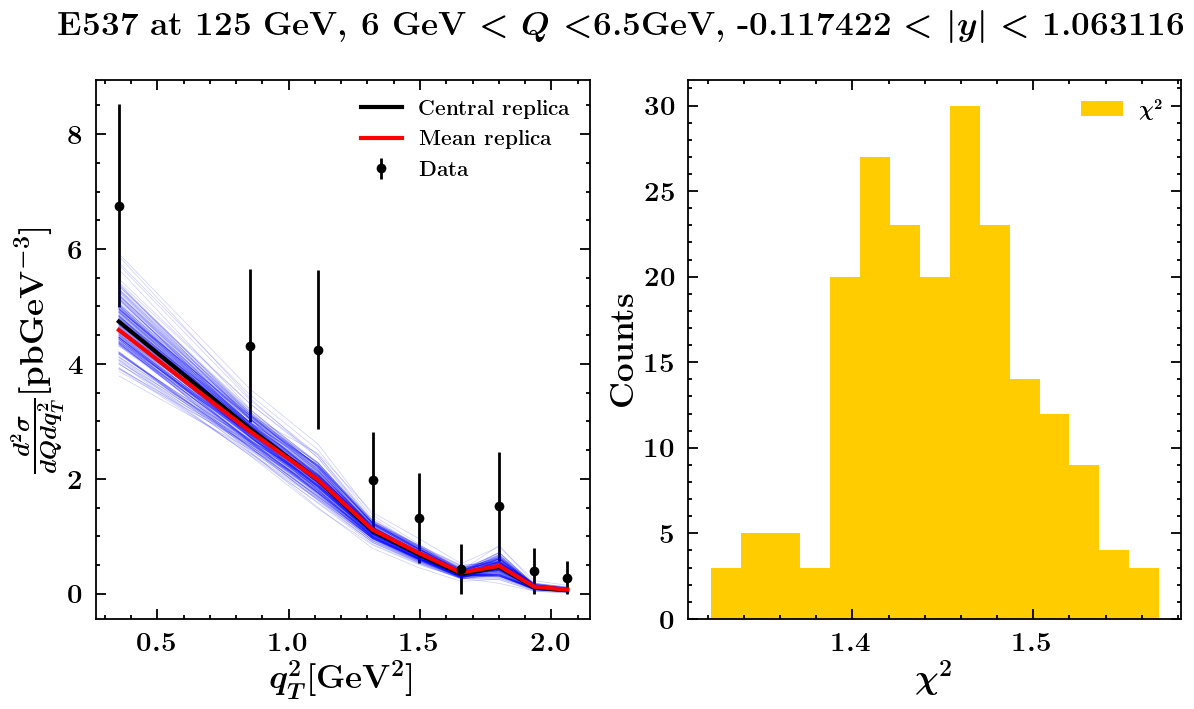
\includegraphics{pngplots/E537_Q_6.0_6.5.png}
\caption{E537\_Q\_6.0\_6.5 data-theory comparison}
\end{figure}

\begin{figure}
\centering
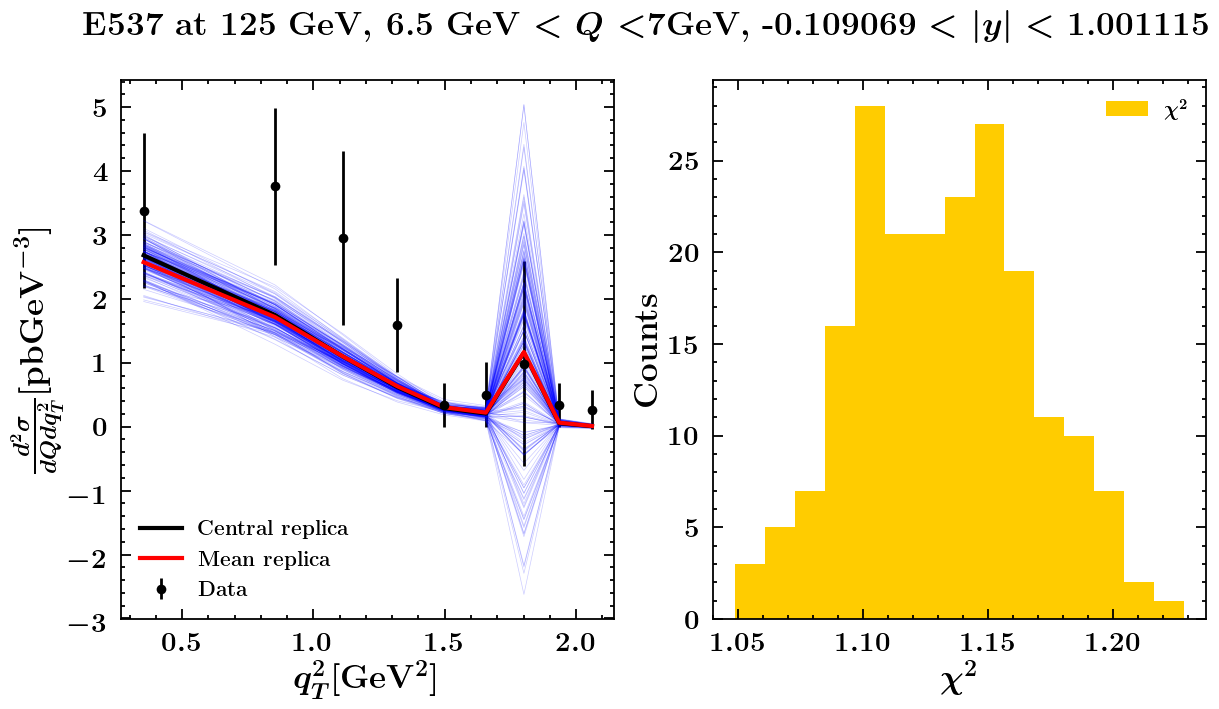
\includegraphics{pngplots/E537_Q_6.5_7.0.png}
\caption{E537\_Q\_6.5\_7.0 data-theory comparison}
\end{figure}

\begin{figure}
\centering
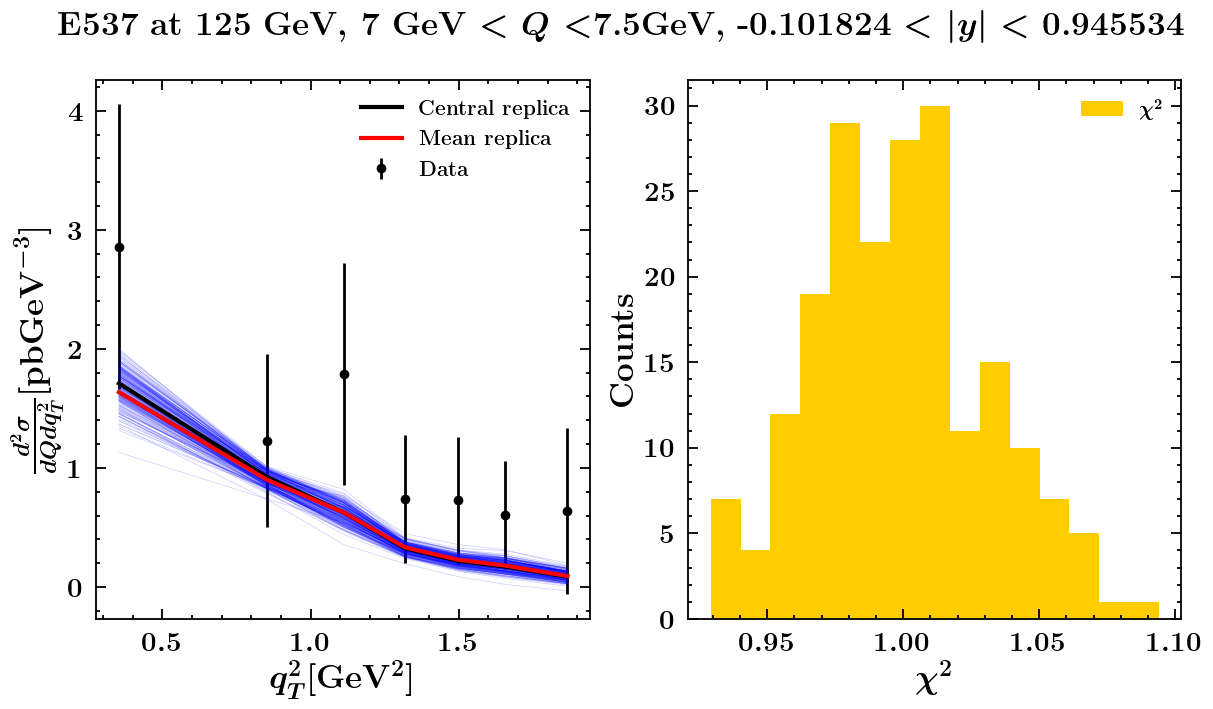
\includegraphics{pngplots/E537_Q_7.0_7.5.png}
\caption{E537\_Q\_7.0\_7.5 data-theory comparison}
\end{figure}

\begin{figure}
\centering
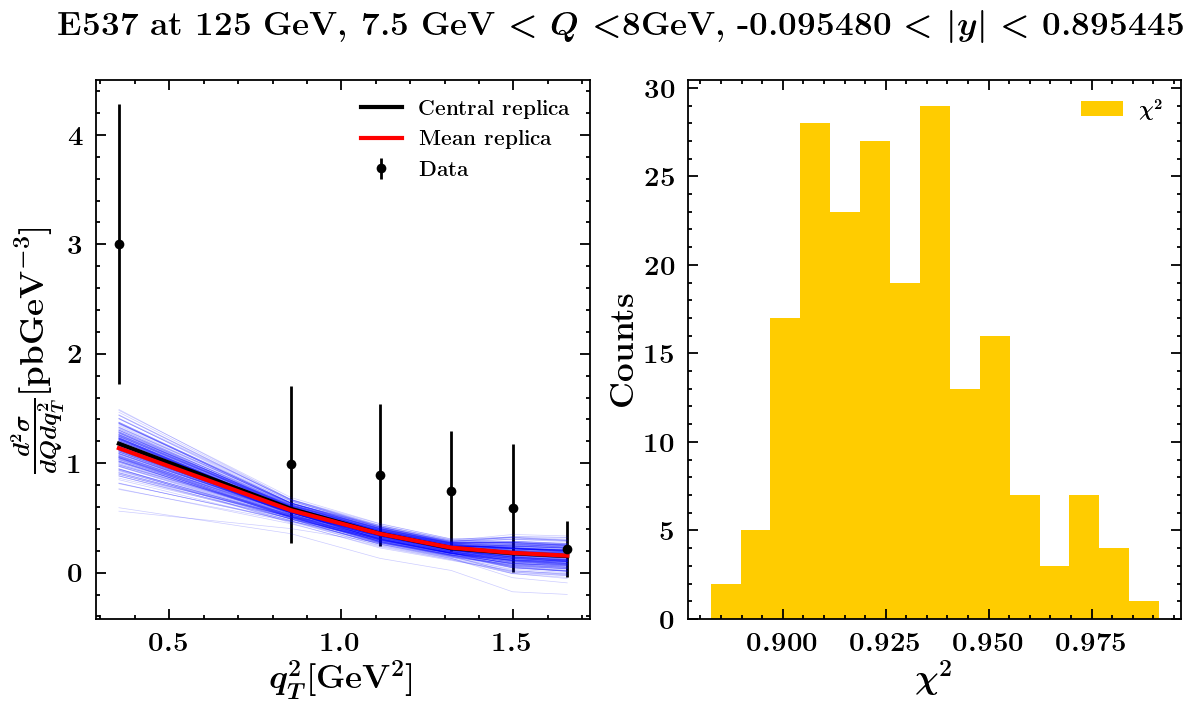
\includegraphics{pngplots/E537_Q_7.5_8.0.png}
\caption{E537\_Q\_7.5\_8.0 data-theory comparison}
\end{figure}

\begin{figure}
\centering
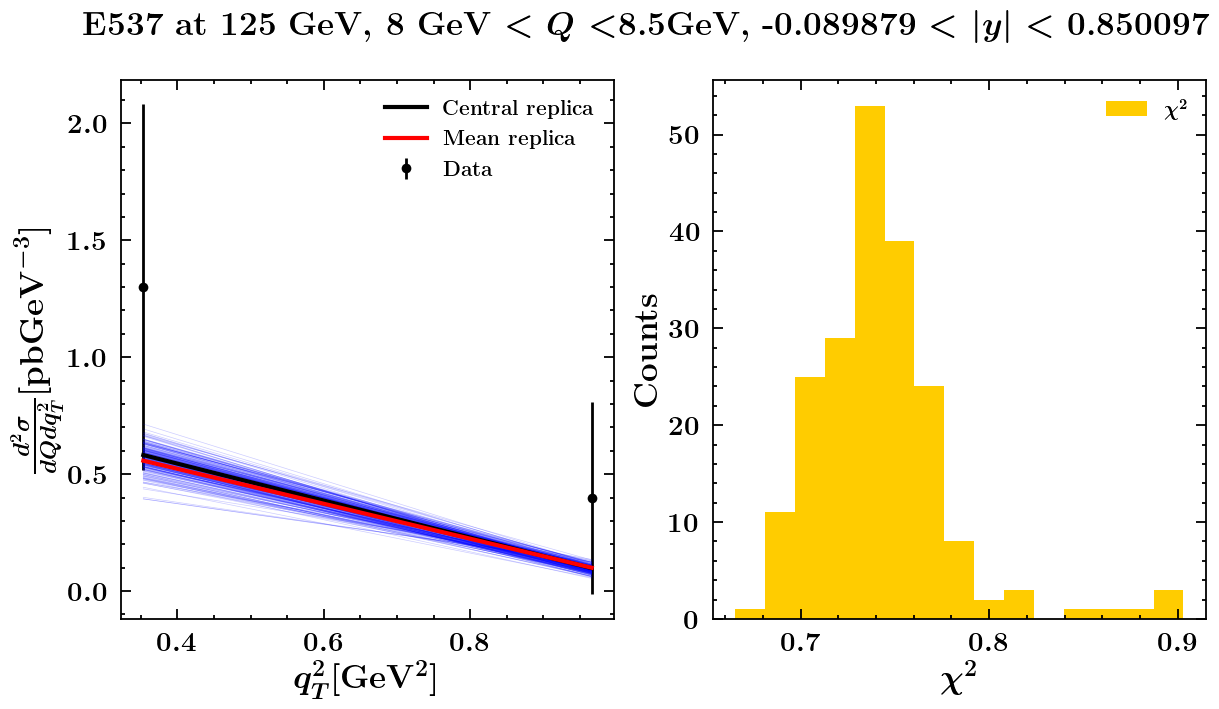
\includegraphics{pngplots/E537_Q_8.0_8.5.png}
\caption{E537\_Q\_8.0\_8.5 data-theory comparison}
\end{figure}

\begin{figure}
\centering
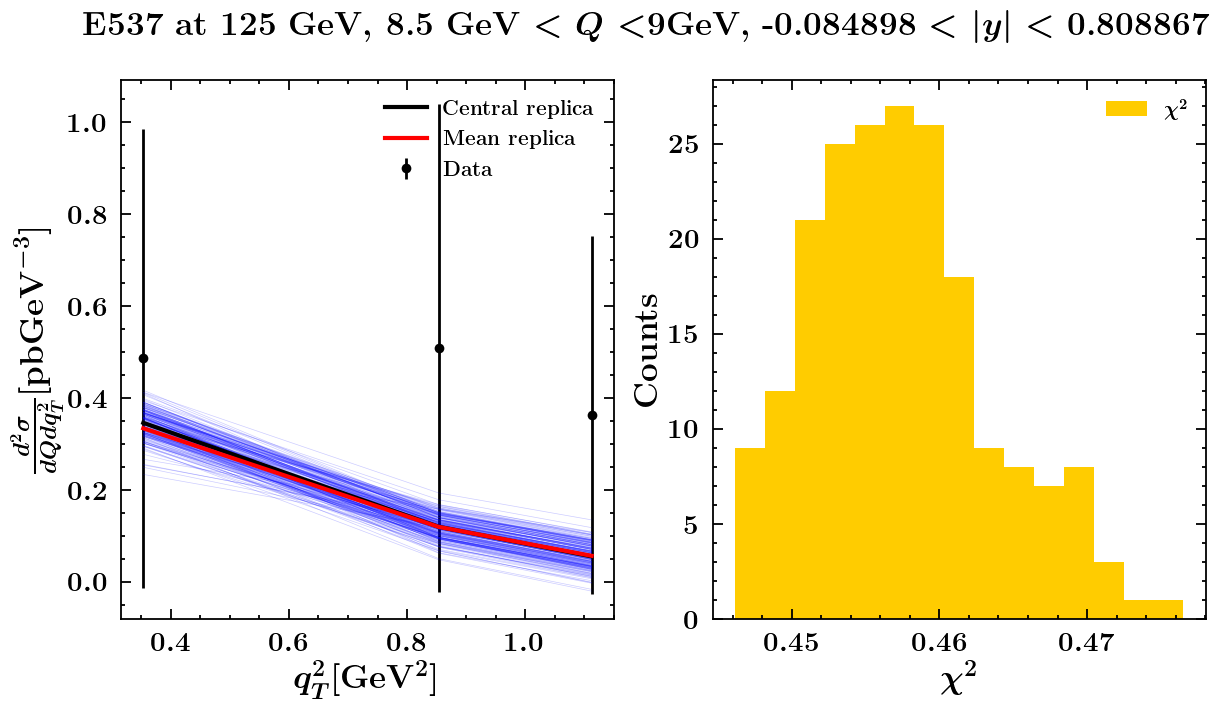
\includegraphics{pngplots/E537_Q_8.5_9.0.png}
\caption{E537\_Q\_8.5\_9.0 data-theory comparison}
\end{figure}

\begin{figure}
\centering
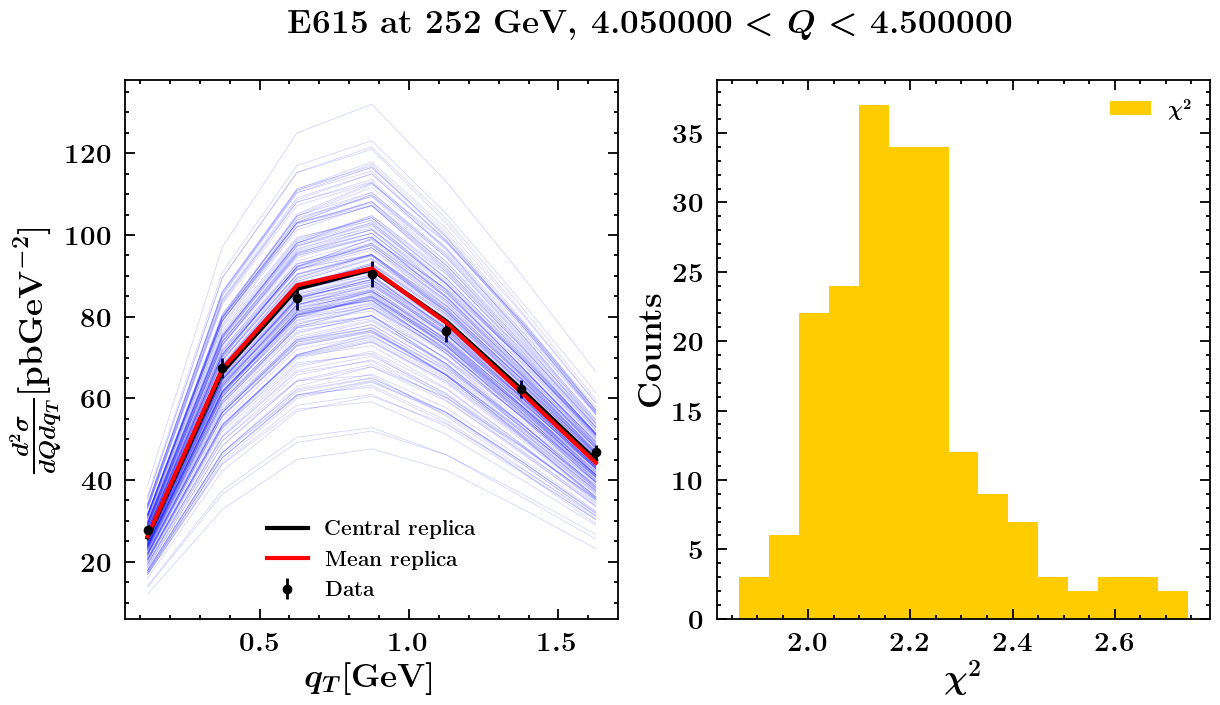
\includegraphics{pngplots/E615_Q_4.05_4.50.png}
\caption{E615\_Q\_4.05\_4.50 data-theory comparison}
\end{figure}

\begin{figure}
\centering
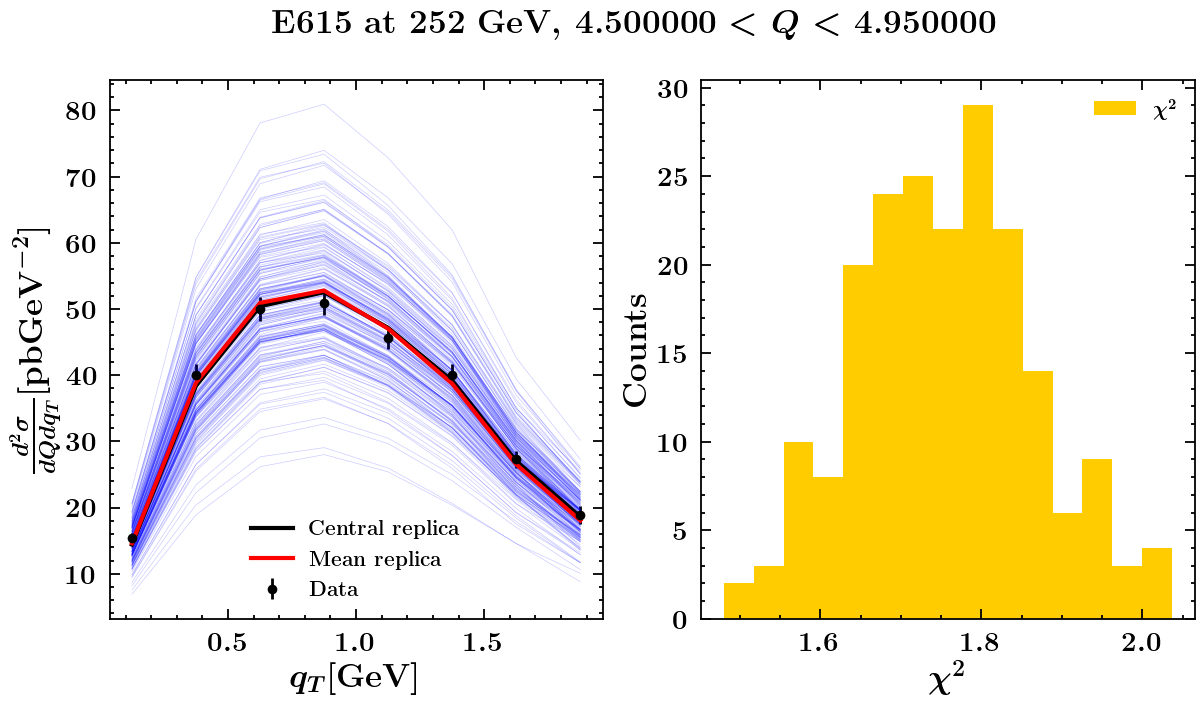
\includegraphics{pngplots/E615_Q_4.50_4.95.png}
\caption{E615\_Q\_4.50\_4.95 data-theory comparison}
\end{figure}

\begin{figure}
\centering
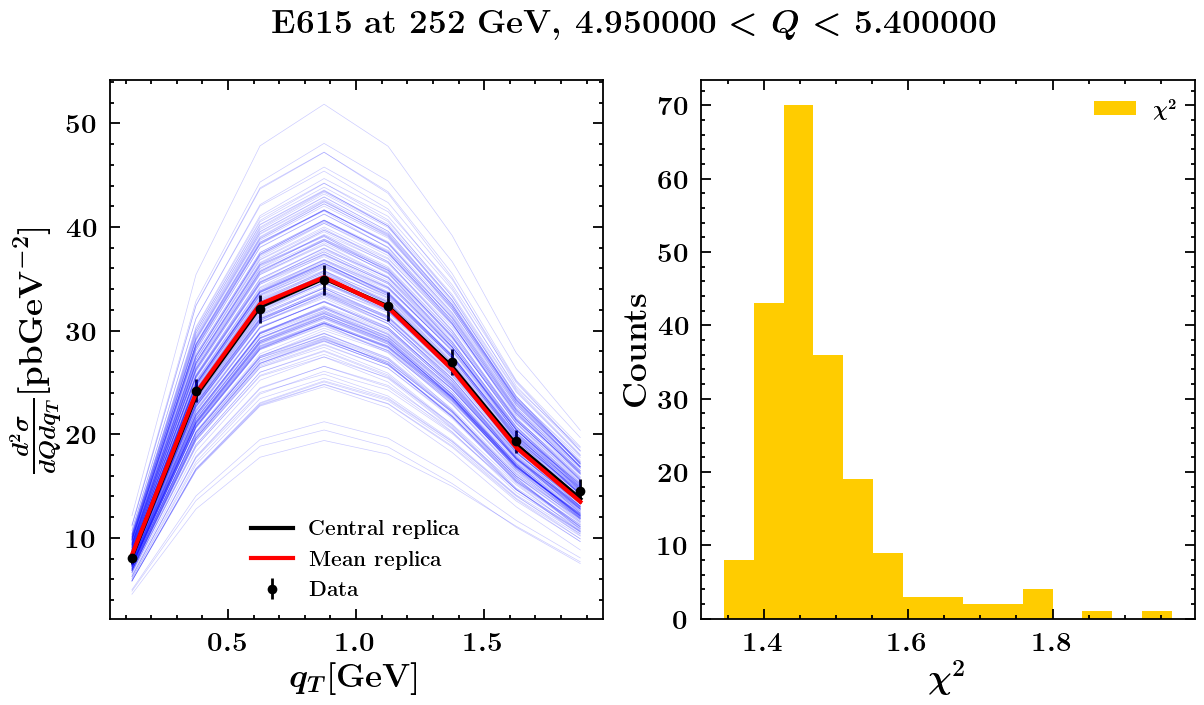
\includegraphics{pngplots/E615_Q_4.95_5.40.png}
\caption{E615\_Q\_4.95\_5.40 data-theory comparison}
\end{figure}

\begin{figure}
\centering
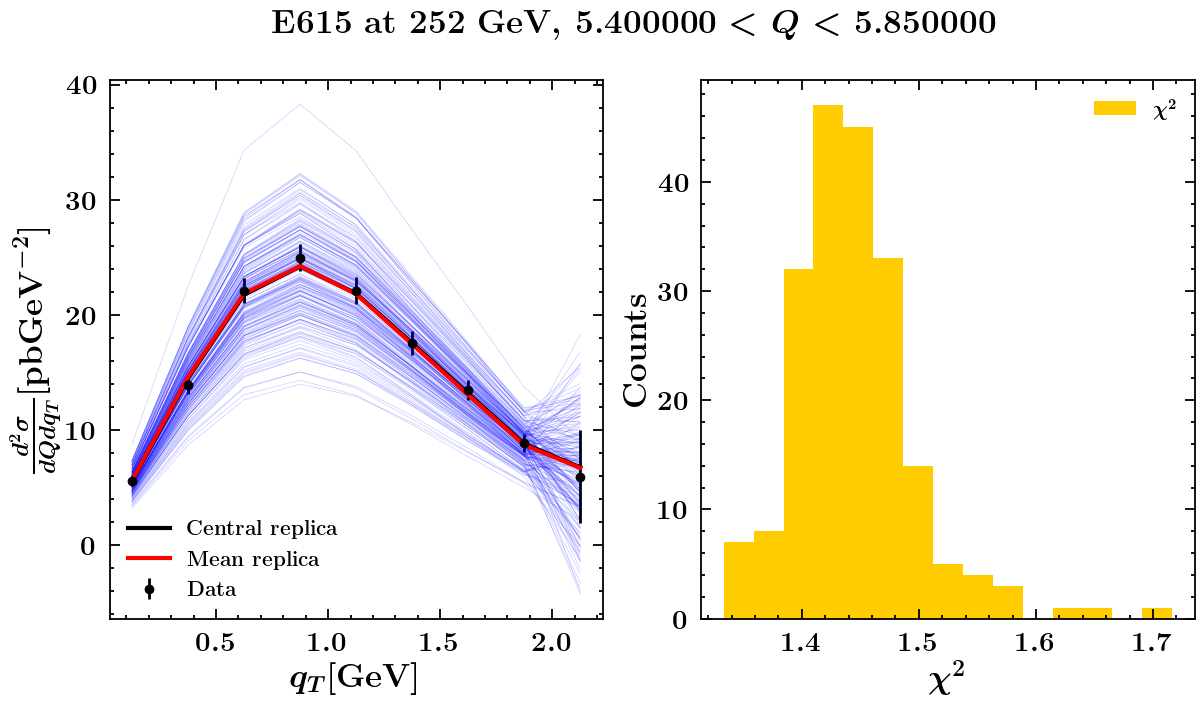
\includegraphics{pngplots/E615_Q_5.40_5.85.png}
\caption{E615\_Q\_5.40\_5.85 data-theory comparison}
\end{figure}

\begin{figure}
\centering
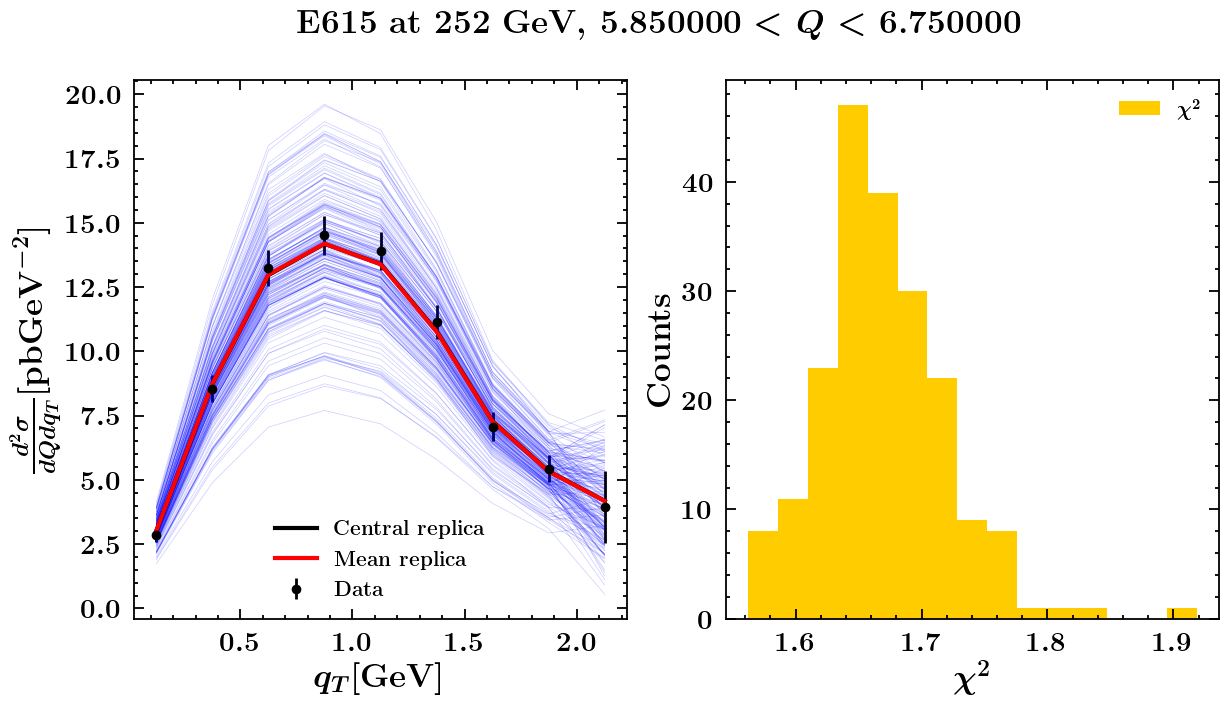
\includegraphics{pngplots/E615_Q_5.85_6.75.png}
\caption{E615\_Q\_5.85\_6.75 data-theory comparison}
\end{figure}

\begin{figure}
\centering
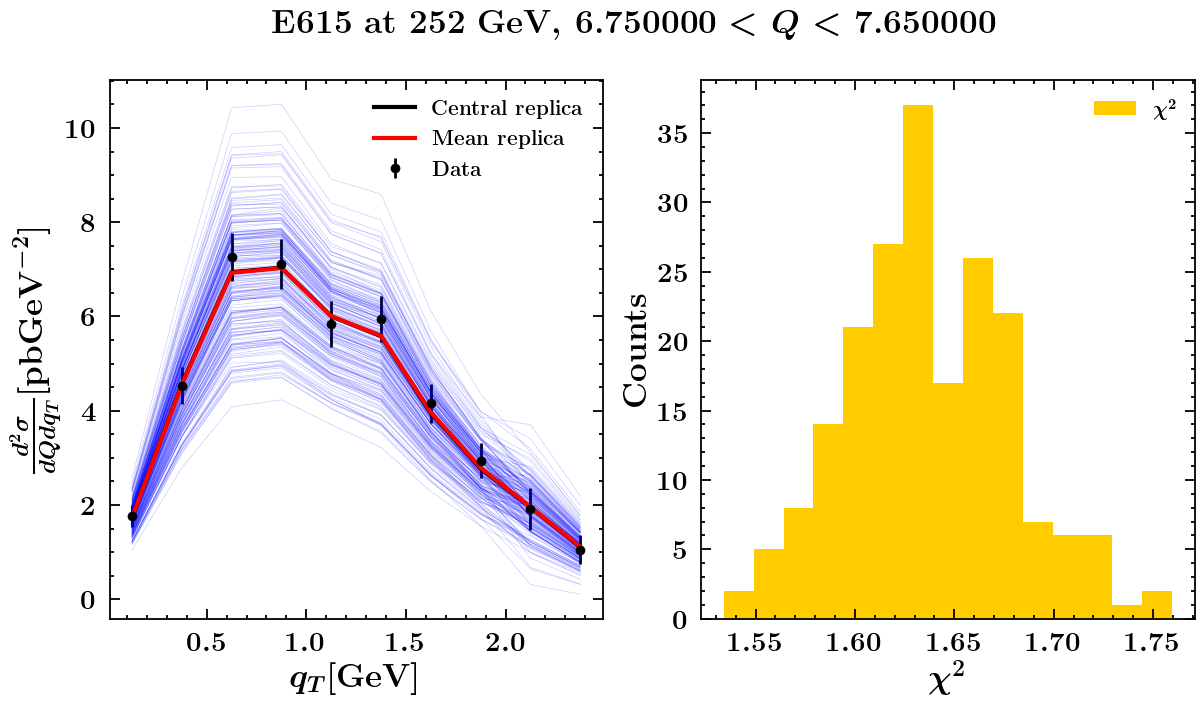
\includegraphics{pngplots/E615_Q_6.75_7.65.png}
\caption{E615\_Q\_6.75\_7.65 data-theory comparison}
\end{figure}

\begin{figure}
\centering
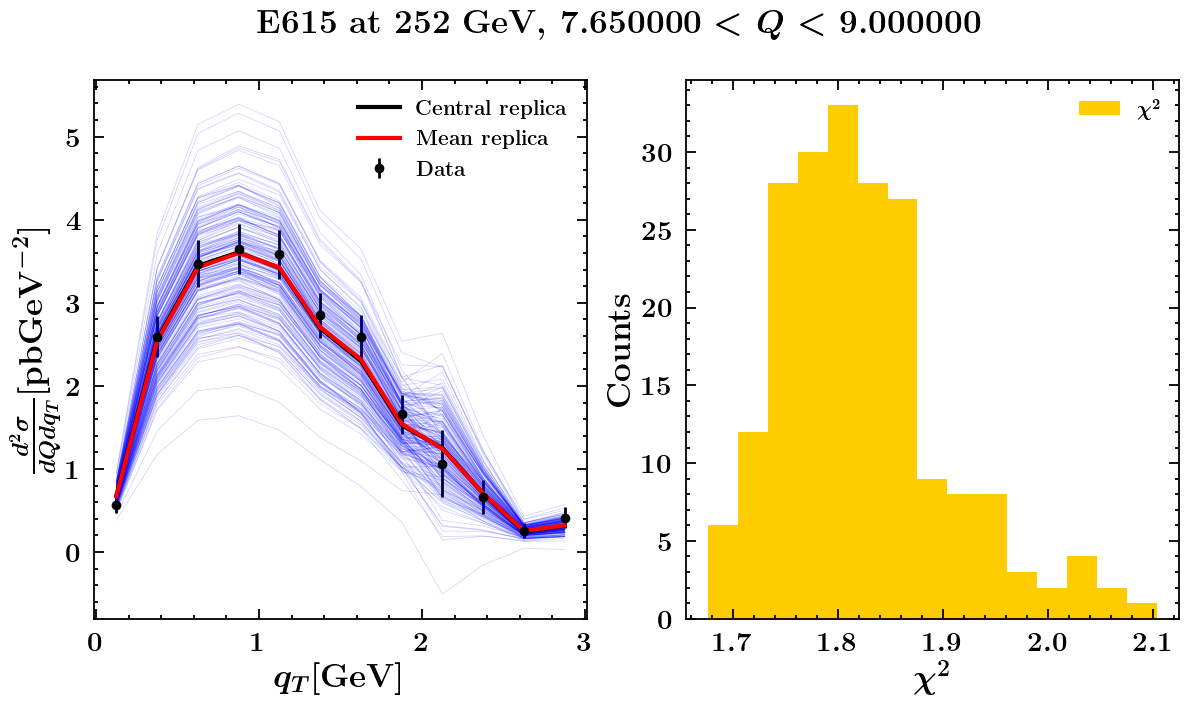
\includegraphics{pngplots/E615_Q_7.65_9.00.png}
\caption{E615\_Q\_7.65\_9.00 data-theory comparison}
\end{figure}

\begin{figure}
\centering
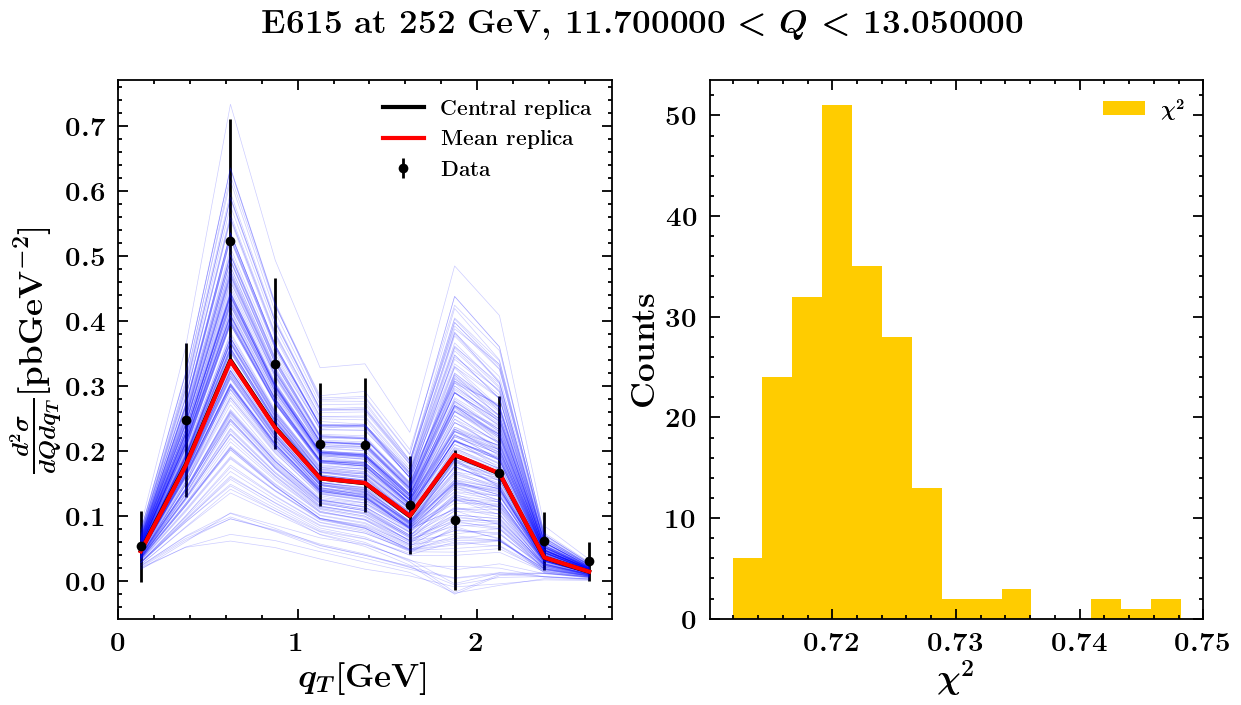
\includegraphics{pngplots/E615_Q_11.70_13.05.png}
\caption{E615\_Q\_11.70\_13.05 data-theory comparison}
\end{figure}

\end{document}
